% Example paper using the example pack's math assets and a pack diagram.
% Build: doc-kit sty example  (once), then  latexmk -pdf paper.tex
\documentclass{article}
\usepackage{graphicx}
\usepackage{ex}          % generated by: doc-kit sty example

\begin{document}

\section*{The heat equation}

The equation and the loss used to fit it are the same assets as on the slides:
\begin{equation}
  \exasset{demo/heat}
  \label{eq:heat}
\end{equation}
With a value for the diffusivity, passed through to the nested asset:
\begin{align}
  &\exasset[kappa=0.1]{demo/heat} \label{eq:heat-01}\\
  &\exasset[kappa=0.1]{demo/residual-loss} \label{eq:loss-01}
\end{align}
Equation~\eqref{eq:loss-01} is the residual of \eqref{eq:heat-01}. Pack macros work too: $\norm{u}$.

\begin{figure}[h]
  \centering
  \IfFileExists{../../src/doc_kit/packs/example/graphics/demo/pipeline.pdf}
    {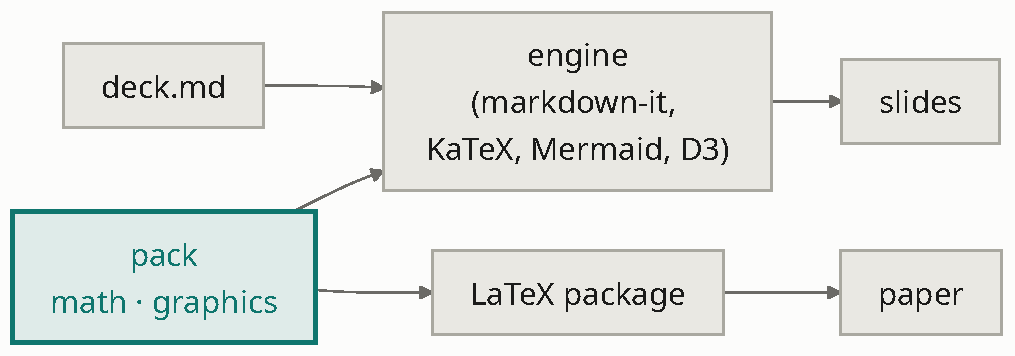
\includegraphics[width=\linewidth]{../../src/doc_kit/packs/example/graphics/demo/pipeline.pdf}}
    {\fbox{run \texttt{doc-kit graphics src/doc\_kit/packs/example} to produce pipeline.pdf}}
  \caption{The pipeline diagram, from the same source as the slides.}
\end{figure}

\end{document}
